\section{Requirements}
\label{sec:Requirements}

\subsection{Overview}
\label{sec:Requirements>Overview}
Initially, this project was conceived by Dr. Kenny Hunt, who served as the advisor, and he gave almost all of the requirements \cite{web:Metropolist} in the first meeting. Both the advisor, who is also the project sponsor, and the developer, who is also the author, are the stakeholders of the project.

\subsection{Functional Requirements}
\label{sec:Requirements>Functional Requirements}
There are two roles for this system: ``admins'' and ``users.'' As a result, the following functional requirements were established for the project:
\begin{enumerate}
  \item As an admin or a user, I need to able to:
  \begin{enumerate}
    \item Log in with a unique email and password
    \item Log out
    \item Edit my personal profile by changing my email, first name, last name, or password
  \end{enumerate}
  \item As an admin, I need to be able to:
  \begin{enumerate}
    \item View all users
    \item Enable or disable any user (not including admins)
    \item Search for a user using any combination of email, username, first name, and last name
  \end{enumerate}
  \item As a user, I need to be able to:
  \begin{enumerate}
    \item Sign up with a unique email, first name, last name, and password
    \item View and search for users
    \item View all of the maps that I have created
    \item View all of the maps shared with me
    \item Search for maps using any combination of the map's name, created date, edited date, the owner's email, the owner's first name, and the owner's last name
    \item Make maps public, private, or viewable by only a select list of users
    \item Download viewable maps in PNG or SVG format
    \item Create a map with a name
    \item Delete a map
    \item Edit a map
    \item Annotate a map
    \begin{enumerate}
      \item Tag buildings with details related to the building
      \item Include virtual-people as owners, residents, or others
      \item Include relationship between virtual-peoples (family, business, sentiments)
    \end{enumerate}
  \end{enumerate}
\end{enumerate}

Figure \ref{fig:Use Case Diagram} is the Use Case Diagram that describes the functionalities to be implemented by this web application.

\begin{figure}[!htbp]
\centering
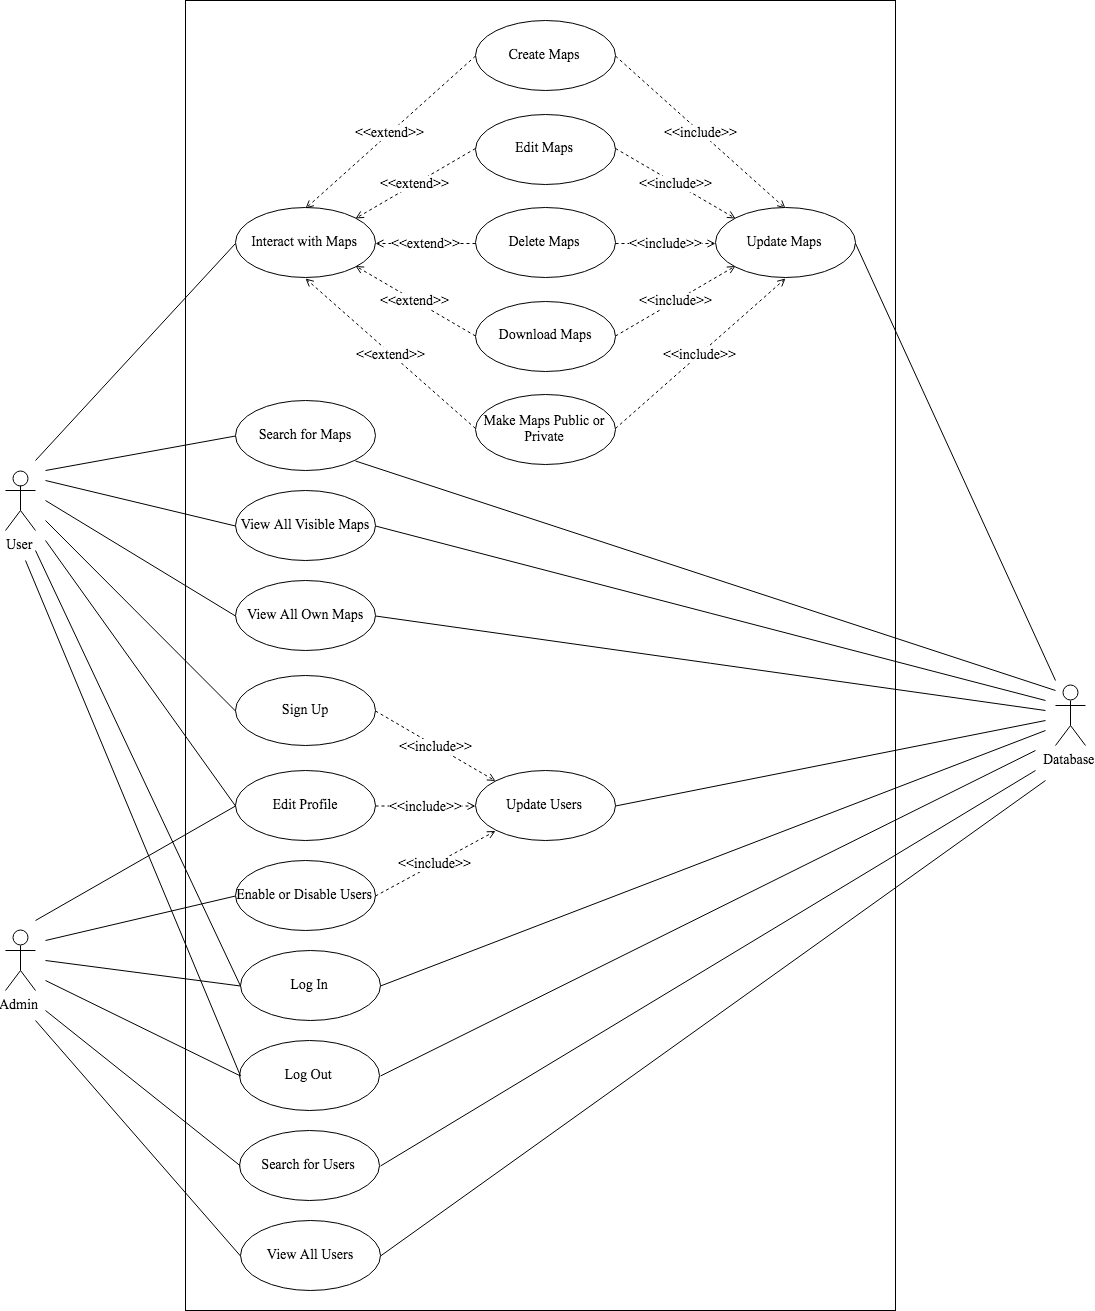
\includegraphics[width=\textwidth]{section02/assets/use_case.png}
\caption[Use Case Diagram]{\label{fig:Use Case Diagram}Use Case Diagram}
\end{figure}

\subsection{Non-Functional Requirements}
\label{sec:Requirements>Non-Functional Requirements}
There are numerous non-functional requirements for this system: response time, availability, usability, security (authentication, authorization, integrity, privacy, etc.), and so on \cite{web:NonFunc}. For this application, we focused on the following requirements:
\begin{enumerate}
  \item Security:
  \begin{enumerate}
    \item Input Validation: All user-supplied data is validated at both client and server

    \item Password Encryption:
    \begin{enumerate}
      \item Password must be encrypted
      \item Not even the system administrators shall see clear text passwords
    \end{enumerate}

    \item Prohibiting Cross Site Scripting (XSS):
    \begin{enumerate}
      \item Never insert data anywhere in a ``script'' element
      \item Never insert data in an HTML comment
      \item Never insert data anywhere in CSS
      \item Never insert data in an attribute name
      \item Never insert data in an attribute value
      \item Never insert data in a tag name
    \end{enumerate}

    \item Secure Session Cookie:
    \begin{enumerate}
      \item Only use secure cookies
      \item Only use ``HttpOnly'' cookies
      \item Always change the session id after login
    \end{enumerate}
  \end{enumerate}

  \item Performance:
  \begin{enumerate}
    \item High performance of rendering map: The map rendering engine must be fast enough to support a viable user experience
  \end{enumerate}
\end{enumerate}

\subsection{Selection of Software Development Life Cycle Model}
\label{sec:Requirements>SDLC}
We identified the following possible risks:
\begin{enumerate}
  \item Lack of experience developing semi-automatic map generation algorithms
  \item Uncertainty regarding third-party libraries that would provide assistance
  \item Potential misunderstanding between the advisor and the developer with respect to the requirements
\end{enumerate}

To reduce or avoid these risks, two life cycle models were considered: Waterfall and Agile. If we use the Waterfall model for software development, then we have to be clear with all the development requirements beforehand as there is no scope of changing the requirements once the project development starts. But for Agile methodology, on the other hand, it provides excellent visibility for key stakeholders, both of the project’s progress and of the product itself, which in turn helps to ensure that expectations are effectively managed. So finally, the Agile model was chosen, which is shown in Figure \ref{fig:Agile Model}.

\begin{figure}[htb]
\centering
\includegraphics[width=\textwidth]{section02/assets/Agile.png}
\caption[Agile Development Life Cycle Model]{\label{fig:Agile Model}Agile Development Life Cycle Model \cite{web:AgileModel}}
\end{figure}

An Agile methodology is a practice that helps continuous iterations of development and testing in the software development process. In this model, development and testing activities are concurrent. Furthermore, the Agile model is a combination of iterative and incremental process models, which breaks the product into small incremental builds. These builds are provided in iterations. Each iteration typically lasts from about one to three weeks.

At the end of each iteration, a working product demo is displayed to stakeholders. There are several known advantages and disadvantages of using the Agile model in this project:
\begin{enumerate}

  \item Advantages:
  \begin{enumerate}
    \item Easy to manage
    \item Little or no planning required
    \item Gives flexibility to developers
    \item Resource requirements are minimum
    \item Suitable for fixed or changing requirements
  \end{enumerate}

  \item Disadvantages:
  \begin{enumerate}
    \item More risks of sustainability, maintainability, and extensibility
    \item An overall plan, an Agile leader (the advisor) is a must without which it does not work
    \item There is a very high individual dependency since there is minimum documentation generated
  \end{enumerate}

\end{enumerate}
